\documentclass{article}

% Language setting
% Replace `english' with e.g. `spanish' to change the document language
\usepackage[italian]{babel}

% Set page size and margins
% Replace `letterpaper' with `a4paper' for UK/EU standard size
\usepackage[letterpaper,top=2cm,bottom=2cm,left=3cm,right=3cm,marginparwidth=1.75cm]{geometry}

% Useful packages
\usepackage{amsmath}
\usepackage{graphicx}
\usepackage{appendix}
\usepackage{siunitx} % Provides the \SI{}{} and \si{} command for typesetting SI units
\usepackage[colorlinks=true, allcolors=black]{hyperref}
\usepackage{caption}
\usepackage{tikz}
\usetikzlibrary{arrows,automata, positioning}

\title{Prova Finale (Progetto Di Reti Logiche)}
\author{Carlo Sgaravatti (Codice Persona 10660072 - Matricola 937539)}
\date{Consegna : 1 Aprile 2022}
\begin{document}
\maketitle
\tableofcontents

%\begin{abstract}
%Your abstract.
%\end{abstract}

\section{Introduzione}

\subsection{Scopo del progetto}

Il progetto è basato sulle codifiche convoluzionali, che sono utilizzate, nell’ambito della trasmissione delle informazioni, per rilevare e correggere gli errori di trasmissione. Nello specifico, l'obiettivo è sviluppare un modulo hardware che implementi un codice convoluzionale 1/2, ovvero: per ogni bit di ingresso vengono generati due bit in uscita.
\newline Il modulo riceve in ingresso una sequenza di n parole da 8 bit, che devono essere codificate in una sequenza di 2n parole da 8 bit. In particolare, si richiede al componente di:
\begin{enumerate}
    \item Leggere il numero di parole da codificare, accedendo ad una memoria RAM
    \item Per ogni parola da codificare:
    \begin{itemize}
        \item leggere la parola dalla memoria RAM
        \item calcolarne la codifica
        \item scrivere il risultato nella memoria RAM
    \end{itemize}
\end{enumerate}
La Figura \ref{fig:convolut} riporta il criterio con cui viene fatta la codifica; in particolare, considerando la sequenza di parole come un'unica sequenza di bit seriali, per ogni bit di ingresso, i bit di uscita sono costruiti nel seguente modo: detto \texttt{u\_k} il bit di ingresso serializzato al tempo k
\begin{itemize}
    \item il primo bit di uscita (\texttt{p\_1k}) è lo xor dell'ultimo e del terzultimo bit della sequenza di ingresso (rispettivamente \texttt{u\_k} e \texttt{u\_k-2})
    \item il secondo bit di uscita (\texttt{p\_2k}) è lo xor degli ultimi tre bit della sequenza d'ingresso (\texttt{u\_k}, \texttt{u\_k-1} e \texttt{u\_k-2})
\end{itemize}

\begin{figure}
\centering
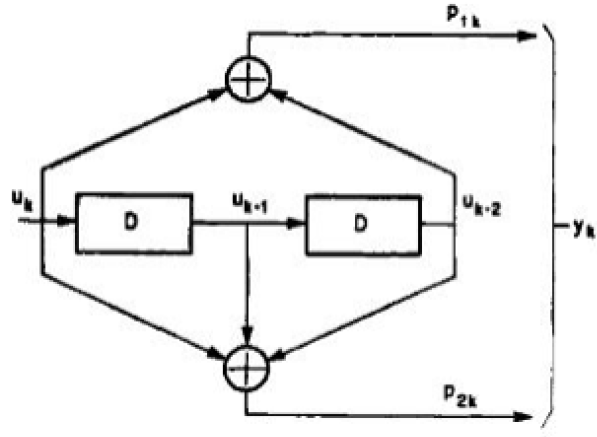
\includegraphics[width=0.5\textwidth]{convolut.png}
\caption{\label{fig:convolut}La codifica dell'uscita}
\end{figure}

\subsection{Interfaccia del componente}
L'interfaccia del componente da descrivere è la seguente:
\texttt{
    \begin{tabbing}
    entit\=y project\_reti\_logiche is \\
    \> port \=(\\
    \> \> i\_clk : in std\_logic;\\
    \> \> i\_rst : in std\_logic;\\
    \> \> i\_start : in std\_logic;\\
    \> \> i\_data : in std\_logic\_vector(7 downto 0);\\
    \> \> o\_address : out std\_logic\_vector(15 downto 0);\\
    \> \> o\_done : out std\_logic\\
    \> \> o\_en : out std\_logic\\
    \> \> o\_we : out std\_logic\\
    \> \> o\_data : out std\_logic\_vector(7 downto 0);\\
    \> );\\
    end project\_reti\_logiche;
    \end{tabbing}
}
Dove:
\begin{itemize}
    \item \texttt{i\_clk} è il segnale di \texttt{CLOCK} in ingresso, generato dal testbench
    \item \texttt{i\_rst} è il segnale di \texttt{RESET} che inizializza la macchina per poter ricevere il primo segnale di \texttt{START} (ovvero la prima sequenza di parole) ed è generato dal testbench
    \item \texttt{i\_start} è il segnale di \texttt{START} generato dal testbench che, quando portato al livello logico alto, fa partire la computazione di una sequenza di parole
    \item \texttt{i\_data} è il segnale (vettore) che arriva dalla memoria in seguito ad una richiesta di lettura
    \item \texttt{o\_address} è il segnale (vettore) di uscita che manda l'indirizzo alla memoria
    \item \texttt{o\_done} è il segnale in uscita che comunica la fine dell'elaborazione della sequenza di parole
    \item \texttt{o\_en} è il segnale di \texttt{ENABLE} da dover mandare alla memoria per potrer comunicare con essa (sia in lettura che in scrittura)
    \item \texttt{o\_we} è il segnale di \texttt{WRITE ENABLE} a dover mandare alla memoria per poterci scrivere (se pari a 1). Per leggere dalla memoria deve essere settato a 0
    \item \texttt{o\_data} è il segnale (vettore) di uscita che contiene la parola da scrivere in memoria
\end{itemize}
Il modulo partirà nell'elaborazione di una sequenza di parole quando \texttt{i\_start} verrà portato ad 1 e terminerà l'elaborazione portando \texttt{o\_done} a 1. Per iniziare una nuova elaborazione, \texttt{i\_start} dovrà essere portato a 0 e si dovrà attendere che \texttt{o\_done} venga portato a 0.

\subsection{Descrizione della memoria}

I dati sono memorizzati in una memoria RAM con indirizzamento al byte, avente la seguente struttura:
\begin{itemize}
    \item l'indirizzo 0 contiene il numero  n di parole da 8 bit contenute nella sequenza di parole da elaborare (con n compreso tra 0 e 255)
    \item gli indirizzi da 1 a n (per n maggiore di 0) contengono le parole da codificare
    \item gli indirizzi da 1000 a (2n - 1) + 1000 sono utilizzati per la scrittura delle parole codificate in uscita dal componente da progettare; in particolare, la codifica dell'i-esima parola in ingresso (contenuta nell'indirizzo i) viene scritta negli indirizzi 2i + 998 e 2i + 999
\end{itemize}
La Figura \ref{fig:mem} riporta un esempio con n = 2.

\begin{figure}
\centering
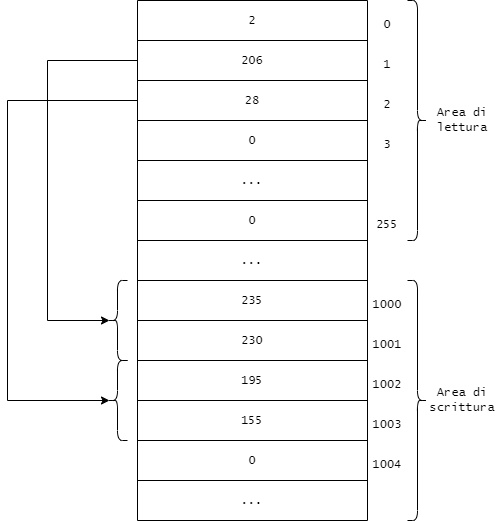
\includegraphics[width=0.7\textwidth]{prov.png}
\caption{\label{fig:mem}Esempio di utilizzo della memoria}
\end{figure}

\section{Architettura}

\subsection{Schema dell'implementazione}
L'architettura è stata progettata in maniera modulare, in particolare sono stati sviluppati i seguenti tre moduli:
\begin{itemize}
    \item \texttt{FSM Principale}: modulo che si interfaccia con la memoria (lettura e scrittura) e che si occupa di gestire il protocollo di inizio e fine della computazione di ogni sequenza di parole (gestito dai segnali i\_start e o\_done). Il modulo rappresenta il top-level component del progetto.
    \item \texttt{Serializzatore/Deserializzatore}: modulo che si occupa di serializzare la parola da elaborare, allo scopo di produrre l'ingresso del Convolutore, e di deserializzare i singoli bit prodotti dal Convolutore per formare le uscite da scrivere in memoria
    \item \texttt{Convolutore}: modulo che si occupa di codificare i singoli bit da produrre in uscita
\end{itemize}
La Figura \ref{fig:tmp2.drawio} mostra uno schema ad alto livello dell'implementazione.
\newline
Tutti e tre i moduli sono macchine a stati ed hanno il medesimo segnale di \texttt{CLOCK}; inoltre, tutte e tre sono realizzate tramite due processi: \texttt{state\_output} e \texttt{delta\_lambda}. Il primo è il processo sequenziale che ha il compito di asserire le uscite e di cambiare lo stato interno sul fronte di salita del clock. Il secondo è il processo combinatorio che calcola le uscite e lo stato interno validi per il prossimo fronte di salita.

\begin{figure}
\centering
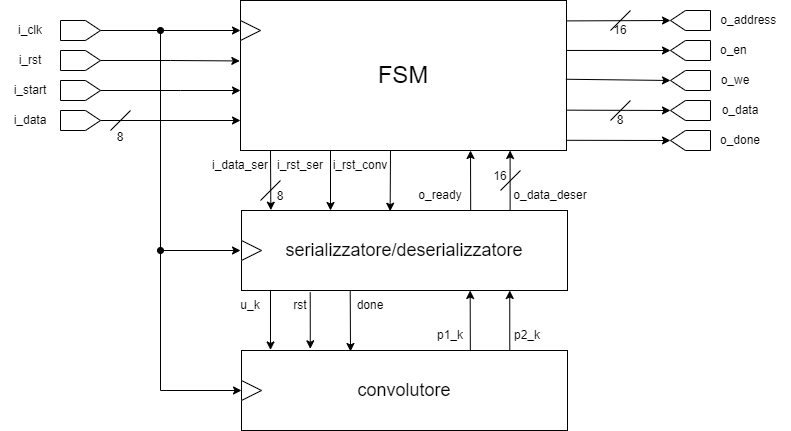
\includegraphics[width=1\textwidth]{tmp2.drawio.png}
\caption{\label{fig:tmp2.drawio}Lo schema ad alto livello dell'implementazione}
\end{figure}

\subsection{FSM principale}
La FSM principale è una macchina a stati avente i seguenti 11 stati:
\begin{itemize}
    \item \texttt{RST}: stato di attesa in cui la macchina aspetta che \texttt{i\_start} venga portato ad 1 per poter iniziare la computazione di una nuova sequenza di parole in ingresso. Nel caso in cui venga alzato \texttt{i\_rst} si ritorna in questo stato.
    \item \texttt{START}: stato in cui viene preparato l'indirizzo iniziale in uscita per poter leggere la lunghezza della sequenza di ingresso. Viene, inoltre, preparato il reset del Convolutore (poiché si è all'inizio di una nuova computazione).
    \item \texttt{READ\_NUM\_BYTE}: stato di attesa della RAM, si aspetta un ciclo di clock per permettere alla RAM di poter asserire l'uscita correttamente.
    \item \texttt{SAVE\_NUM\_BYTE}: stato in cui si salva all'interno di un registro a 8 bit, detto \texttt{num\_word\_in}, il valore contenuto nella prima cella di memoria della RAM, che rappresenta il numero di parole in ingresso. Tale registro servirà poi per identificare la fine della computazione della sequenza di parole.
    \item \texttt{SET\_ADDR}: stato in cui si prepara l'indirizzo di memoria dal quale verrà letta la prossima parola. L'indirizzo di lettura viene memorizzato nel registro \texttt{o\_address\_read} e, prima di modificarlo (viene incrementato di uno ad ogni lettura), gli 8 bit meno significativi di tale registro vengono confrontati con \texttt{num\_word\_in}: se essi sono uguali allora la computazione è finita in quanto sono già state lette tutte le parole.
    \item \texttt{READ\_WORD}: stato in cui si attende che la RAM asserisca l'uscita correttamente.
    \item \texttt{SAVE\_WORD}: stato in cui la parola in uscita dalla RAM viene salvata nel registro a 8 bit \texttt{data\_ser}, che costituirà l'ingresso del Serializzatore nel ciclo di clock successivo . In questo stato viene inoltre preparato il reset del serializzatore (il quale, dal ciclo di clock, successivo, inizierà a serializzare la parola in ingresso). 
    \item \texttt{CALC\_OUT}: stato in cui si attende che la codifica delle due parole da scrivere in RAM sia pronta. La codifica della parola viene salvata in un apposito registro a 16 bit, detto \texttt{o\_data\_tmp}, che conterrà la concatenazione delle due parole da scrivere in memoria.
    \item \texttt{MEM\_WRITE\_FIRST}: stato in cui si prepara la scrittura della prima parola in memoria (contenuta in \texttt{o\_data\_tmp(15 downto 8)}), la cui scrittura effettiva avverrà nel ciclo di clock successivo.
    \item \texttt{MEM\_WRITE\_SECOND}: stato in cui si prepara la scrittura della seconda parola in memoria (contenuta in \texttt{o\_data\_tmp(7 downto 0)}), la cui scrittura effettiva avverrà nel ciclo di clock successivo.
    \item \texttt{DONE}: stato che sancisce la fine della computazione. In questo stato, il segnale \texttt{o\_done} viene portato al livello logico alto e rimane tale fino a che il segnale \texttt{i\_start} non diventa 0.
\end{itemize}
Di seguito è riportato il diagramma degli stati, dove sono state fatte le seguenti abbreviazioni per alcuni degli stati:
\begin{center}
\begin{tabular}{ll}
\texttt{READ\_NUM\_BYTE}: & \texttt{READ\_NB} \\
\texttt{SAVE\_NUM\_BYTE}: & \texttt{SAVE\_NB} \\
\texttt{SET\_ADDR}: & \texttt{SET\_ADD} \\
\texttt{READ\_WORD}: & \texttt{READ\_WR} \\
\texttt{SAVE\_WORD}: & \texttt{SAVE\_WR} \\
\texttt{MEM\_WRITE\_FIRST}: & \texttt{MEM\_WR1} \\
\texttt{MEM\_WRITE\_SECOND}: & \texttt{MEM\_WR2} \\
\end{tabular}
\end{center}

\begin{center}
\begin{tikzpicture}[->,>=stealth',shorten >=1pt,auto,node distance=2cm,
                    semithick, initial where=above, initial text={\texttt{RESET}}]

  \tikzstyle{every state} = [font=\small]
  \node[initial,state] (A)                    {\texttt{RST}};
  \node[state]         (B) [below of=A] 	  {\texttt{START}};
  \node[state]         (C) [below of=B] 	  {\texttt{READ\_NB}};
  \node[state]         (D) [below of=C] 	  {\texttt{SAVE\_NB}};
  \node[state]         (E) [below of=D]       {\texttt{SET\_ADD}};
  \node[state]         (F) [right=4cm of E]       {\texttt{READ\_WR}};
  \node[state]         (G) [below of=F]       {\texttt{SAVE\_WR}};
  \node[state]         (H) [below of=G]       {\texttt{CALC\_OUT}};
  \node[state]         (I) [left=4cm of H]       {\texttt{MEM\_WR1}};
  \node[state]         (J) [below of=I]       {\texttt{MEM\_WR2}};
  \node[state]         (K) [left=4cm of C]       {\texttt{DONE}};

  \path (A) edge              node [pos=0.5]{\texttt{i\_start=1}} (B)
 	    (A) edge [loop right] node {} (A)
        (B) edge              node {} (C)
        (C) edge              node {} (D)
        (D) edge 			  node {} (E)
        (E) edge 			  node {} (F)
        (E) edge [bend left]  node [pos=0.5]{\texttt{num\_word\_in=o\_address\_read(7..0)}} (K)
        (F) edge 			  node {} (G)
        (G) edge 			  node {} (H)
        (H) edge [loop right] node {} (H)
        (H) edge              node [pos=0.5]{\texttt{o\_ready=1}} (I)
        (I) edge 			  node {} (J)
        (J) edge [bend left]  node {} (E)
        (K) edge [bend left]  node [pos=0.5]{\texttt{i\_start=0}} (A)
        (K) edge [loop left]  node {} (K)
        (E);
        
\end{tikzpicture}
\end{center}
\captionof{figure}{Diagramma degli stati della Macchina a Stati Finiti}

%\newpage

\subsection{Serializzatore/Deserializzatore}

L'interfaccia del Serializzatore/Deserializzatore è la seguente:
\texttt{
    \begin{tabbing}
    entit\=y serializzatore\_deserializzatore is \\
    \> port \=(\\
    \> \> i\_data\_ser : in std\_logic\_vector(7 downto 0);\\
    \> \> i\_rst\_ser : in std\_logic;\\
    \> \> i\_clk : in std\_logic;\\
    \> \> i\_rst\_conv : in std\_logic;\\
    \> \> o\_data\_deser : out std\_logic\_vector(15 downto 0);\\
    \> \> o\_ready : out std\_logic\\
    \> );\\
    end serializzatore\_deserializzatore;
    \end{tabbing}
}
In particolare:
\begin{itemize}
    \item \texttt{i\_data\_ser} è il byte da serializzare, proveniente dalla memoria
    \item \texttt{i\_rst\_ser} è il segnale di \texttt{RESET} del serializzatore
    \item \texttt{i\_clk} è il segnale di \texttt{CLOCK} ed è lo stesso della FSM principale
    \item \texttt{i\_rst\_conv} è il segnale di \texttt{RESET} del Convolutore, che viene propagato dal Serializzatore/Deserializzatore verso il Convolutore
    \item \texttt{o\_data\_deser} è un segnale a 16 bit che forma il concatenamento delle due parole da scrivere in memoria alla fine dell'elaborazione di \texttt{i\_data\_ser} da parte del Convolutore
    \item \texttt{o\_ready} è il segnale che notifica la fine dell'elaborazione del byte alla FSM principale
\end{itemize}
La presenza di due segnali di \texttt{RESET} è dovuta al fatto che il Serializzatore/Deserializzatore e il Convolutore devono esser resettati in due momenti diversi: il primo deve essere resettato quando inizia la computazione di una nuova parola, il secondo quando inizia la computazione di una nuova sequenza di parole. I due segnali vengono entrambi asseriti dalla FSM principale in maniera sincrona, dunque non avverrà mai un reset asincrono né del Serializzatore/Deserializzatore né del Convolutore.
\newline La macchina a stati esegue un ciclo di conteggio da 0 a 9:
\begin{itemize}
    \item il ciclo da 0 a 7 si occupa di serializzare il dato in ingresso, fornendo il bit di ingresso del convolutore: quando il conteggio è 0 si prepara il bit più significativo di \texttt{i\_data\_ser} (ovvero \texttt{i\_data\_ser(7)}) come ingresso del Convolutore, quando il conteggio è 7 si prepara il bit meno significativo di \texttt{i\_data\_ser} (ovvero \texttt{i\_data\_ser(0)}) come ingresso del Convolutore; dunque, al ciclo di conteggio i viene preparato \texttt{i\_data\_ser(7-i)} come ingresso del Convolutore. Poichè la modifica del'ingresso vero e proprio del Convolutore avviene sul fronte di salita del clock, la computazione effettiva del Convolutore avviene nel ciclo di conteggio da 1 a 8.
    \item il ciclo da 2 a 9 si occupa di raccogliere i due bit di uscita del Convolutore nel segnale \texttt{o\_data\_deser}; i bit vengono deserializzati in \texttt{o\_data\_deser} partendo dal bit più significativo (\texttt{o\_data\_deser(15)}).
\end{itemize}
Alla fine del conteggio, il modulo porta il segnale \texttt{o\_ready} a 1, dunque la macchina si mantiene nello stesso stato (senza produrre nuovi ingressi per il Convolutore) fino a che non avviene un reset. Inoltre, il modulo comunica con il Convolutore tramite un segnale \texttt{done}, che viene alzato quando il conteggio è 8 (e viene mantenuto alto fino a quando il conteggio non ritorna a 0 ) e che notifica al Convolutore di non modificare più le sue uscite e il suo stato interno fino a quanto tale segnale non ritorna a 0.

\subsection{Convolutore}

Il Convolutore è una macchina a stati avente la seguente interfaccia:
\texttt{
    \begin{tabbing}
    entit\=y convolutore is \\
    \> port \=(\\
    \> \> u\_k : in std\_logic;\\
    \> \> clk : in std\_logic;\\
    \> \> rst : in std\_logic;\\
    \> \> done : in std\_logic;\\
    \> \> p1\_k : out std\_logic;\\
    \> \> p2\_k : out std\_logic\\
    \> );\\
    end convolutore;
    \end{tabbing}
}
Dove:
\begin{itemize}
    \item \texttt{u\_k} è il bit d'ingresso da codificare
    \item \texttt{clk} è il segnele di \texttt{CLOCK}
    \item \texttt{rst} è il segnale di \texttt{RESET}
    \item \texttt{done} è un segnale proveniente dal Serializzatore/Deserializzatore: se è 1 allora la serializzazione è finita, dunque il Convolutore non cambia più il suo stato e non modifica più le sue uscite, se è a 0 allora il Convolutore si comporta normalmente
    \item \texttt{p1\_k} e \texttt{p2\_k} sono i due bit di uscita, che rappresentano la codifica di \texttt{u\_k}.
\end{itemize}
La Figura \ref{fig:conv} riporta il diagramma degli stati del Convolutore, considerando \texttt{done} pari a 0.

\begin{figure}
\centering
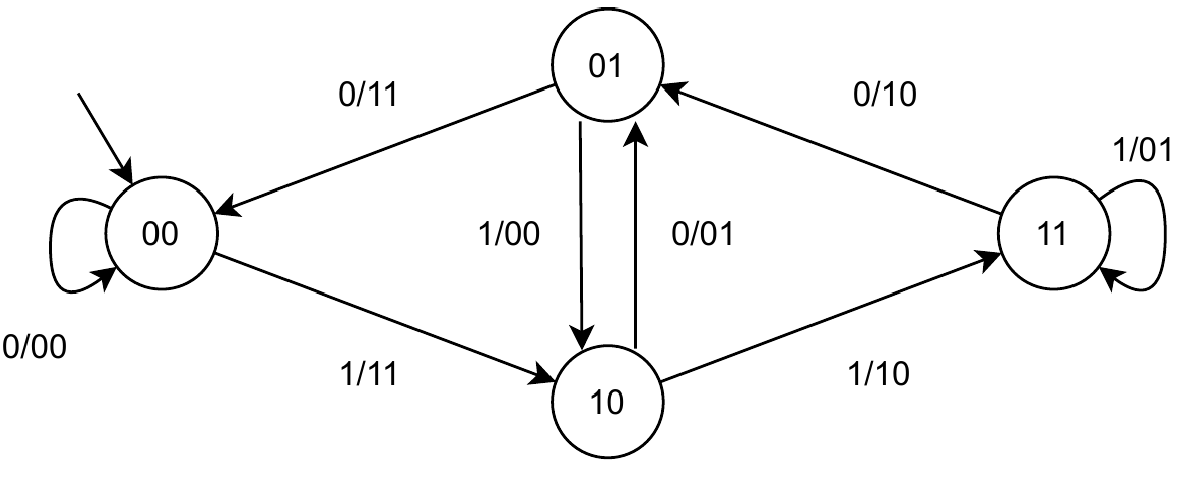
\includegraphics[width=0.9\textwidth]{conv.png}
\caption{\label{fig:conv}Il diagramma degli stati del Convolutore con  \texttt{done} uguale a 0}
\end{figure}

\subsection{Scelte progettuali e ottimizzazioni}

L'architettura è stata realizzata in maniera modulare per poter per poter separare le funzionalità di calcolo della codifica, di serializzazione della parola di ingresso e di interfacciamento con la memoria; questo ha permesso di parallelizzare la serializzazione e il calcolo della codifica dell'uscita.
\newline Le ottimizzazioni hanno riguardato soprattutto la FSM principale; in particolare, si è scelto di utilizzare un set di registri per memorizzare l'indirizzo di lettura della memoria (incrementato di uno ad ogni lettura) e di non memorizzare l'indirizzo di scrittura, in quanto quest'ultimo viene ricavato da quello di lettura. Questo ha permesso di risparmiare sull'utilizzo di qualche registro, poiché l'eventuale memorizzazione dell'indirizzo di scrittura richiederebbe ulteriori registri per poterlo incrementare di 1 ad ogni scrittura. 
\newline Un'ulteriore ottimizzazione riguarda il processo di scrittura: la scrittura effettiva in memoria della seconda parola avviene quando la FSM principale si trova nello stato \texttt{SET\_ADDR}, in questo modo la scrittura della parola e la preparazione dell'indirizzo di memoria successivo da cui leggere avvengono nello stesso stato; lo stesso avviene anche con la prima parola da scrivere, che viene scritta in memoria quando la FSM principale sta preparando l'indirizzo di scrittura della seconda parola da scrivere. Questo ha consentito di risparmiare due cicli di clock per ogni parola da codificare in uscita.

\section{Risultati sperimentali}

\subsection{Report di sintesi}

Il componente risulta correttamente simulabile con l'utilizzo di 144 Lookup Tables e di 100 Flip Flop, come lo si può notare dalla Figura \ref{fig:report_utilizzo}. Si è fatta particolare cautela nella scrittura del codice per evitare l'uso di Latch.

\begin{figure}
\centering
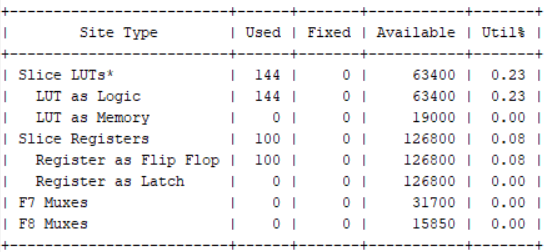
\includegraphics[width=0.7\textwidth]{utilization_report.png}
\caption{\label{fig:report_utilizzo}Il report di utilizzo}
\end{figure}

\subsection{Simulazioni}
Sono stati effettuati alcuni test per verificare condizioni di funzionamento ritenute significative; in particolare, oltre al testbench d'esempio, sono stati scritti i seguenti testbench:
\begin{itemize}
    \item Indirizzo 0 della RAM contenente la parola "00000000": test che rappresenta il caso limite in cui la lunghezza della sequenza di ingresso è nulla
    \item Segnale di \texttt{RESET} asincrono: il segnale di reset viene asserito dal testbench nel mezzo della computazione, con l'obiettivo di verificare che la macchina riprenda la computazione dall'inizio
    \item Lunghezza della sequenza di ingresso pari a 255: l'obiettivo del test è verificare se il modulo progettato è in grado di gestire il caso limite in cui la lunghezza della sequenza di ingresso è massima
    \item Due sequenze di parole: test che mira a verificare il corretto funzionamento del protocollo per la gestione più sequenze di parole
\end{itemize}
Oltre ai test descritti, sono stati usati anche ulteriori testbench generati casualmente, mantenendo la validità della specifica. Per tutti i test è stata effettuata la simulazione behavioral ed in seguito le simulazioni functional e timing post-synthesis, tutte con successo. Si è, inoltre, provato a variare anche il periodo di clock: il componente ha mantenuto il suo funzionamento anche a 1 ns nella simulazione Functional Post-Synthesis e a 5 ns nella simulazione Timing Post-Synthesis.

\section{Conclusioni}

Si ritiene che il componente progettato rispetti la specifica, il che è stato verificato mediante testing estensivo sia in pre-sintesi che in post-sintesi. I test effettuati hanno evidenziato alcune criticità nella soluzione iniziale, consentendo di sviluppare la soluzione fino alla sua versione finale. Lavorare alla soluzione dei problemi ha permesso di comprendere bene il funzionamento di Vivado e di migliorare la capacità di risolvere i problemi in maniera efficiente. In particolare, l'analisi delle forme d'onda è stata importante per sviluppare al meglio il progetto.

\end{document}